\documentclass[12pt]{article}
\usepackage[utf8]{inputenc}
\usepackage{mathptmx}
\usepackage{float}
\usepackage{lastpage}
\usepackage{natbib}
\usepackage{graphicx}
\usepackage[margin=1.1in]{geometry}
\usepackage{listings} 
\usepackage[]{mcode}
\usepackage{watermark}
\usepackage{blindtext}
\usepackage{amsmath}
\usepackage{graphicx}
\usepackage{float}
\usepackage{footnote}
\usepackage{multirow}
%\makesavenoteenv{table}
\usepackage[bottom]{footmisc}
\usepackage{mathpazo}
\usepackage{subfig}
\usepackage{mathtools}
\usepackage{animate}
\usepackage[justification=centering]{caption}
\usepackage{wrapfig}
\usepackage{lipsum}
\usepackage{url}
\usepackage{breakurl}
\usepackage[breaklinks]{hyperref}

\usepackage{fancyhdr}
\pagestyle{fancy}
\lhead{Howdy}
\rhead{42490 TEMO}


\linespread{1.5} % Line spacing

% \setlength\parindent{0pt} % Uncomment to remove all indentation from paragraphs

\graphicspath{{./Pictures/}} % Specifies the directory where pictures are stored

\usepackage{geometry}
 \geometry{
 a4paper,
 total={170mm,257mm},
 left=30mm,
 right=30mm,
 top=20mm,
 bottom=20mm
 }
 
\begin{document}

%\renewcommand{\headrulewidth}{0.4pt} %header


\cfoot{\thepage\ of \pageref{LastPage}}
%-------------------------------------------------------------------------------
%	TITLE PAGE
%-------------------------------------------------------------------------------
\begin{titlepage}

\newcommand{\HRule}{\rule{\linewidth}{0.5mm}} % Defines a new command for the horizontal lines, change thickness here

\center % Center everything on the page


\includegraphics[width=0.1\textwidth]{DTU-logo.pdf}
\quad \quad \quad \quad 

\includegraphics[width=0.3\textwidth]{Logo_NoSubtitle_BlueGrey.png}
\\[0.5cm]




\textsc{\large 42490 Technology, management, organisation and Business models}\\[0.5cm] % Minor heading such as course title

%\textsc{\large \bfseries Tennis Major Tournament Match Statistics}\\[0.5cm]

\HRule \\[0.8cm]
{ \huge \bfseries HOWDY - WorklifeBarometer\\[0.4cm] % Title of your document
\HRule \\[1cm]

\begin{minipage}{0.5\textwidth}
\begin{center} \small
\emph{Team - "No group name"}\\
\emph{TAs - Kasper \& Lars}
\begin{table}[H]
\centering
\resizebox{0.5\textwidth}{!}{%
\begin{tabular}{|l|l|}
\hline
\multicolumn{1}{|c|}{\textbf{Student number}} & \multicolumn{1}{c|}{\textbf{Responsible for}} \\ \hline
s144211 & 1.2, 1.3 \\ \hline
 Kazi & 2.2 \\ \hline
s193100 & 1.1 \\ \hline
 &  \\ \hline
 &  \\ \hline
 &  \\ \hline
\end{tabular}%
}
\end{table}
\end{center}
\end{minipage}\\[4cm]

\thiswatermark{\centering \put(-180,-720){
\includegraphics[scale=0.55]{DTU-frise-SH-15.pdf}} }
}


% Signatures, we might have to remove the name part and just keep the student nr
% I am unsure of this since the pp is contradicting itself 
\begin{tabular}{cc}
 $\overline{\qquad\text{s153986}\qquad}$ \quad& \quad
 $\overline{\qquad\text{s144211}\qquad}$ \\ [1cm]
 $\overline{\qquad\text{s154328}\qquad}$ \quad& \quad
 $\overline{\qquad\text{s193100}\qquad}$ \\[1cm]
  $\overline{\qquad\text{(s number)}\qquad}$ \quad& \quad
 $\overline{\qquad\text{(s number)}\qquad}$ \\
\end{tabular}\\[1cm]

{\small
\today %dato 
}
\\[0.2cm] % Date, change the \today to a set date if you want to be precise



\end{titlepage}

\newpage
\tableofcontents

\newpage
\section{PART I : Present situation - MARCO}

% How to comment 
% 2-3 pages !
% 1.How would you characterise the company based on the presentation?
% 2.What is/are the key problem(s)? (be aware that the key problem(s) is not necessarily identical with the challenge and might only be implicitly given in the challenge).
% 3.What is the consequence of the present situation?
% 4.What impact does the situation have on the three organisational levels?
% 5.Who is/are the problem owner(s)?
% Use models and theories to describe the context of the company, strategy, organisational design, business models etc
% Combine these models and theories with the data presented in the company challenge.


Worklife Barometer ApS is a Danish Startup Established in 2014, born with the purpose of preventing sick leaves, by adopting a validated questionnaire for the identification of wellbeing. Its strategy is based on interposing itself between the companies and their employees to guarantee a more fluid dialog on personal matters.     
In order to reach this achievement, it proposes three kinds of products regarding different wellbeing aspects: Howdy wellbeing, Howdy body and Howdy feedback.\cite{howdywebsite}

\noindent Howdy Wellbeing is based on a schema of 5 questions, asked to the employees 2 times a month.
Furthermore, it gives, in real time, an overview of their status, underlining the first symptoms of sickness.
When a sign of stress is detected, Howdy proceeds by making a psychologist call the stressed employee to offer assistance and to guide them. This is done with the purpose of avoiding a worsening of the situation.

\noindent Often companies do not have the right resources, or they do not know how to organize annual surveys for their employees. For this reason, Howdy offers Howdy feedback,[4] to collect employees’ opinions anytime the company deems it necessary.

\noindent Currently, Howdy is composed of more than 10 employees skilled in IT, sales, marketing and product development and supported by external professionals (psychologists and physiotherapists). Worklife Barometer ApS is boasting 14000 users spared on approx. 70 companies, (such as Simens, Skat, Scania, Orsted and Københavns commune) between Denmark, Sweden and the United Kingdom. Their goal is to reach new customers and to expand to other countries in the next years.\cite{howdywebsite}. Thanks to Howdys product and service, 1.6\% of sick leaves have been prevented and 12\% of the users claimed that it has led them to talk to their manager about wellbeing-problems. \cite{howdywebsite}  

\noindent Even though Howdy is gathering positive feedback from its customers, it has been observed that they have not managed to on-board enough customers and are currently losing money. In the following report, Howdy will be analyzed in order to detect the reasons why.

\noindent In particular it has been asked to focus on GTM (go-to-make) strategy, especially on pricing strategy, and to identify the right team (in terms of roles) that will bring the company to a further step.\cite[s.39]{oneofthepresentations}

\noindent In this report, business models will be used in an attempt to look at Howdy from different perspectives. This should draw a wider and more clear picture of the company. Thereby, it will be possible to inspect the company at all levels and to point out possible improvements. This study will start with the identification of the key problem and a problem owner, which are:


\begin{itemize}
  \item key problem : HOWDY is not successfully getting new clients and scaling the business\cite[s.38]{oneofthepresentations}
  \item problem owner: Rasmus Hartung (CEO)\cite[s.5]{oneofthepresentations}
\end{itemize}





\subsection{Assumptions}

While doing the analysis and building up the solution, a couple of assumptions were made. These are:

\begin{enumerate}
    \item Howdy have the resources to hire new people 
    \item The bonus plan for the sales department is adequate 
    \item Howdy has not been marketing sufficiently 
\end{enumerate}

\noindent As Howdy has mentioned plans of expanding the sales team they should have resources to hire new people.

\noindent Howdy has a bonus plan for the sales team that we believe motivates the sales team to sell Howdy’s product and the teams performance should therefore be adequate.

\noindent Howdys marketing is focused on pushing their product through partners like the pension companies but these companies only run campaigns for their own product and Howdy is not allowed to participate. This means that they pretty much are dependent on their partners who do not increase on-boarding of customers at a particularly fast rate. We acknowledge that a much larger campaign and negotiation with pension companies regarding the promotion of Howdy’s product can develop the marketing strategy.


\newpage
\section{PART II : Retrospective analysis}
% 5-7 pages !
% Identify and analyse causal explanations to the key problem(s) rooted in managerial, business and organisational issues:
% Choose one organisational level as your starting point and make it clear who “owns” the key problem(s).
% Argue why the chosen starting point is relevant in order to identify and analyse causal explanations.
% Select and introduce models and theories to be used and motivate why the chosen focus on the challenge is relevant.
% Make your analysis and outline the causes, relevant actors, opportunities, threats, strengths, weaknesses etc.

% THIS IS ALSO WRITTEN BY NIPUN

A \textbf{retrospective analysis} or \textbf{retrospective study} is a research method that is used when the outcome of an event is already known.\\
\noindent In this section an analysis of the current state of Howdy is presented. The reason for executing a retrospective analysis is to create a clear image of what problems Howdy are facing and what causes are leading to these problems.\\
\noindent The models implemented are purely based on the company’s presentation and feedback session from 2019.



\subsection{STAR model}
The star model is a tool that makes the user present the organizational framework of a company and allows this framework to be analysed and evaluated. In this case the star model is used to present the foundation of the company to the reader and to identify potential problems within the different elements of the company’s framework and any inconsistencies between these elements. These problems can then be backed up by other models that are more specific to the part wherein the problem is identified.

\noindent \textbf{Strategy} $|$ Howdy has competitors in their market and must therefore differentiate from them. The main difference between Howdys' product and their competitors' is that they have a focus on the mental health of the client’s employees where their competitors mainly focus on the performance of the employee and how to optimize it. Howdy is mostly targeting white collar businesses as they generally have more capital than other companies that they can invest in products like the one Howdy is offering.
Howdy listens to the market and adapts their product with improvements or new features as they discover new needs or wants from their customers. This can be seen in their products Howdy body and Howdy feedback which have been developed after their main product Howdy wellbeing.

\noindent \textbf{Structure} $|$ The company has a flat organizational structure like many other smaller companies and start-ups. This usually means that there is a foundation for good communication between the different departments. It can be challenged by the fact that most of the employees work from home, but it seems like the distance between co-workers is handled by daily meetings that are both work related and for casual conversation. The structure also plays a part in one of the problems within the company. Namely that employees working in development end up helping with maintenance as there are not enough resources in the department. This slows down development of the product which is a key factor in starting up and growing a technology-based company.

\noindent \textbf{Processes} $|$ As discussed in the previous part most of the employees of Howdy are working from home. This posses a challenge with communication. They seem to have overcome day-to-day communication but there is still no way for the management to check up on the working hours and performance of the employees which can cause problems with employee performance. The single employee hired specifically for maintenance can not handle the workload from maintaining the systems for the current customers which results in the developers having to help. This interrupts the development process which has a high priority within the company’s strategy of adapting to the market.

\noindent \textbf{Rewards} $|$ Howdy has one reward system in place in the form of a bonus plan for their sales staff.

\noindent \textbf{People} $|$ Howdy is a small company employing a little over 10 people. The bookkeeping is outsourced to Exacta Revision and they also use external psychologists for their operation which can be increasing the cost for Howdy.
The company has a department of two people in Sweden consisting of a country manager and a client- and marketing manager. It is not known if they are successful in getting any customers in Sweden.
The sales department consists of a sales director and a client manager which is most likely insufficient if they want to push their products and scale their business.


\subsection{Business model canvas}
A business model canvas is a design for the successful operation of a business. It illustrates how to create value while delivering products or services to your customers. In this report, the business model canvas was used to provide a description of how Howdy creates, delivers, and captures value to its customers. The business model canvas is divided into 9 sections, each responsible for the most vital business elements of every organization. By understanding these elements, we can recognize areas that Howdy can be improved in order to rebuild the organizational innovative strategy. The BMC for Howdy was developed using information given by Howdy in their presentation \cite{oneofthepresentations} and can be seen below in figure \ref{fig:BCmodel}.

\begin{figure}[H]
\centering
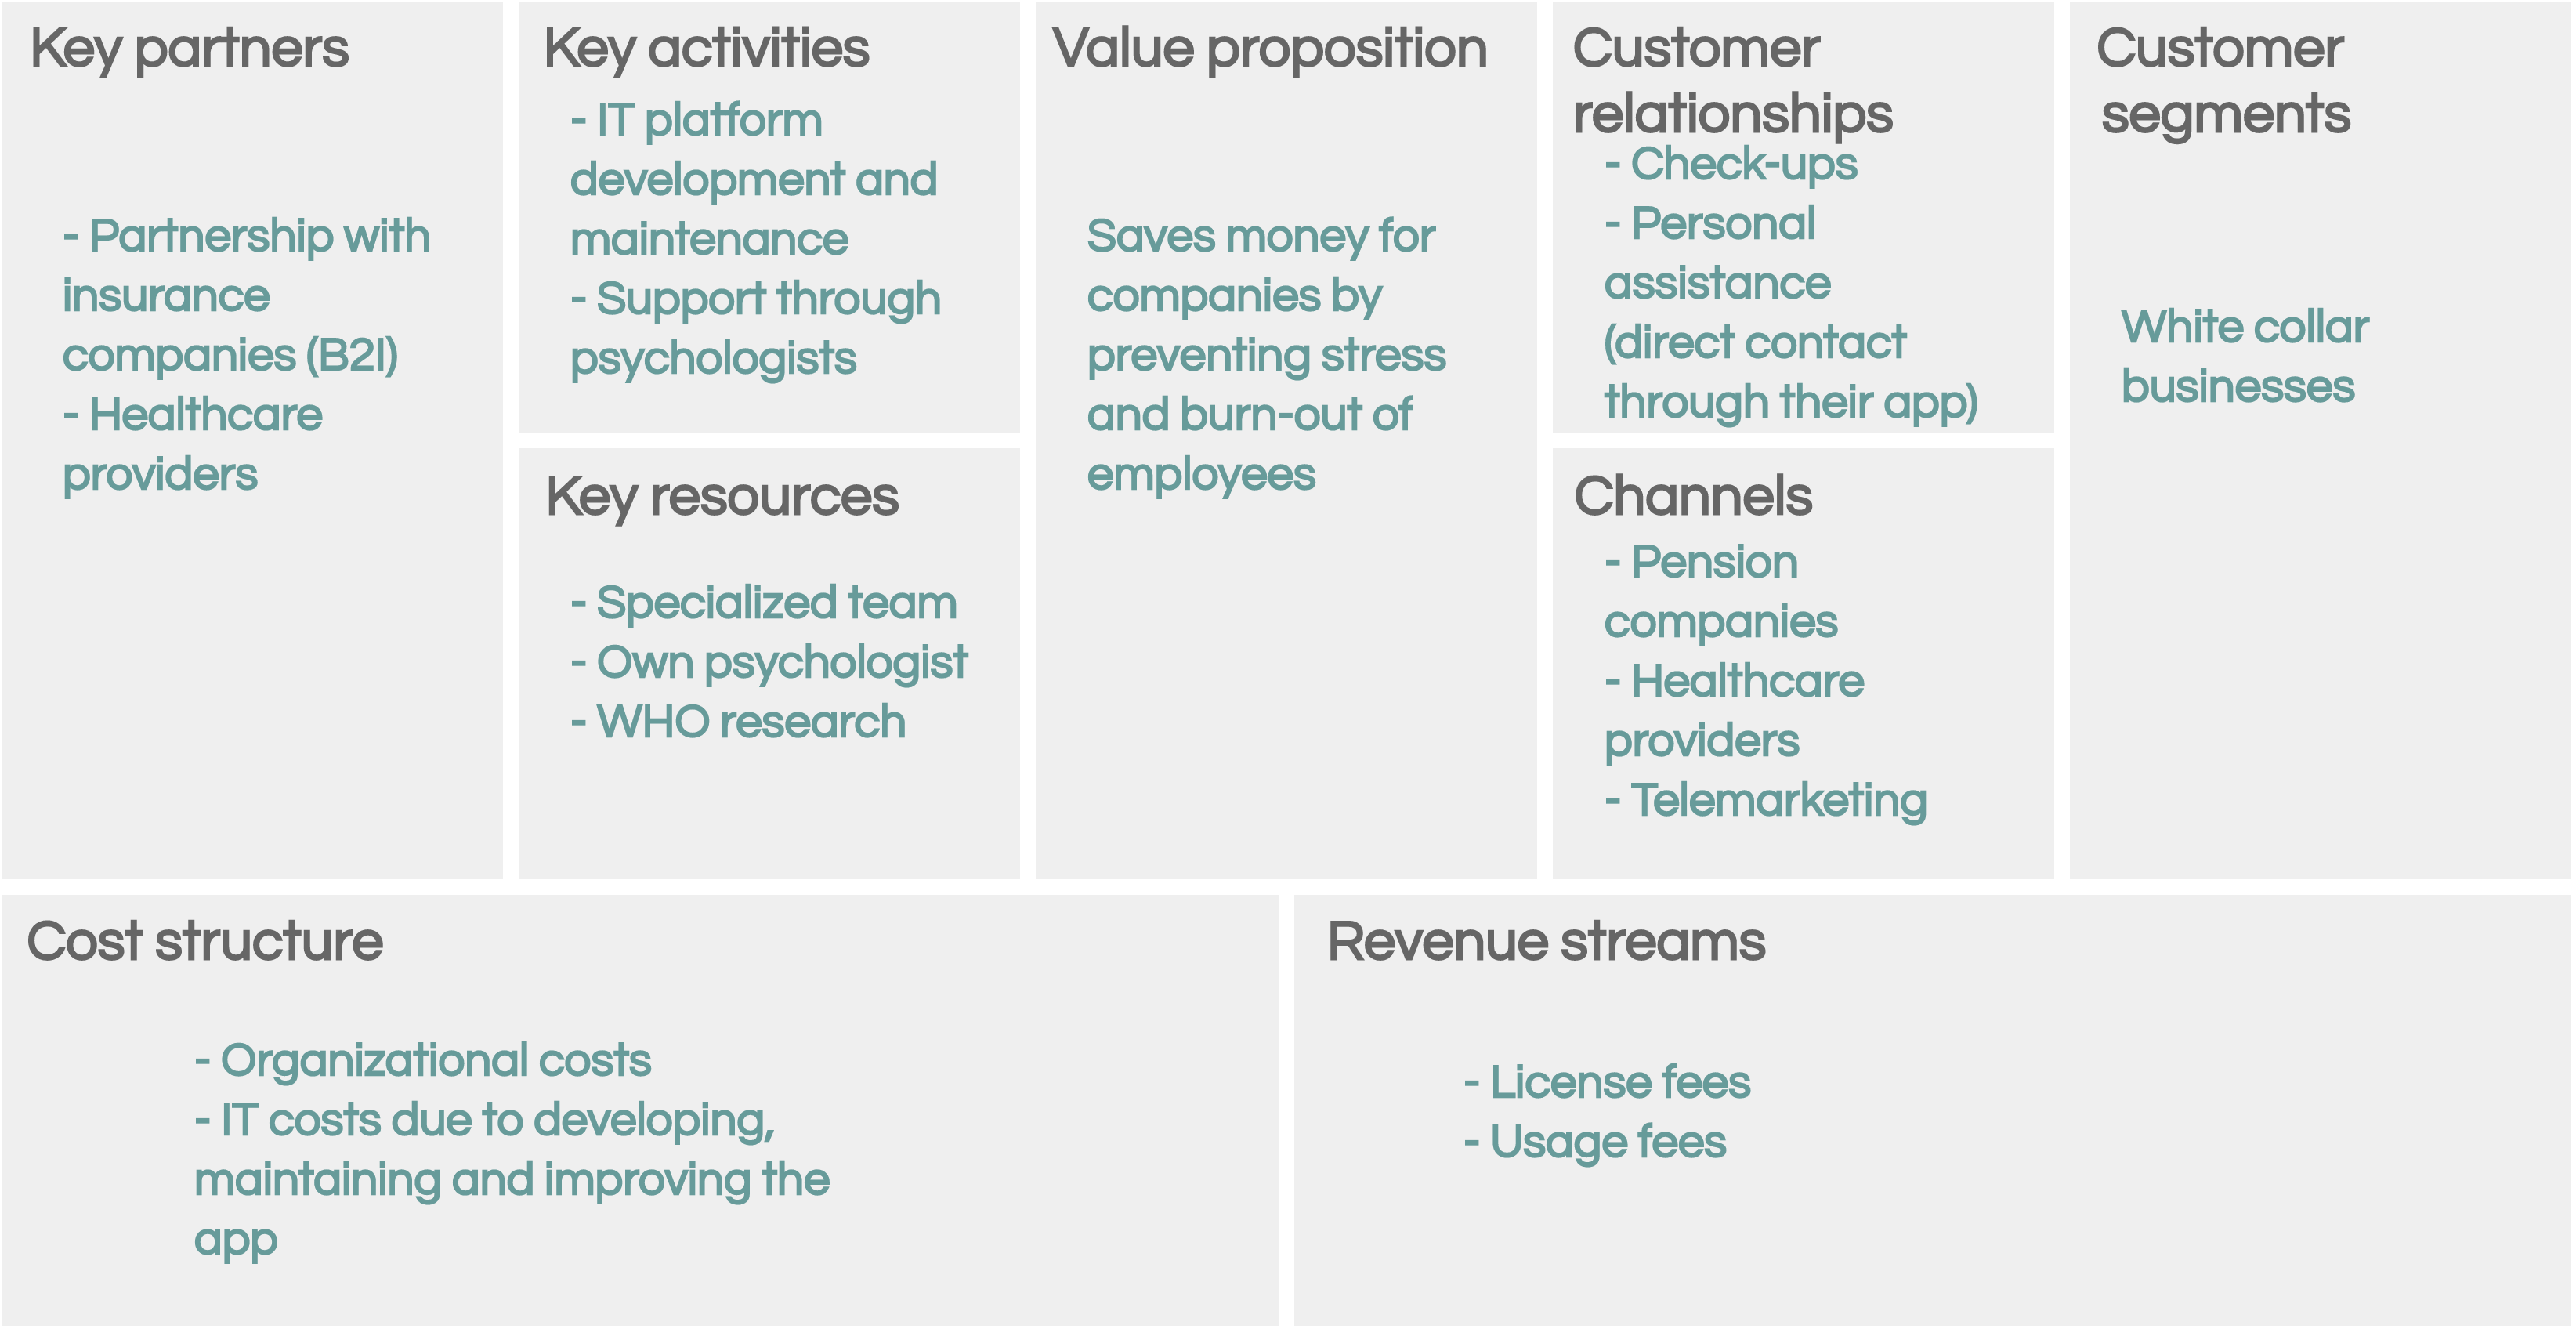
\includegraphics[width=14cm]{figures/BMC3.png}
\caption{Howdy - Business Model Canvas}
\label{fig:BCmodel}
\end{figure}

\noindent \textbf{Key Partners} $|$ The key partners of Howdy includes Insurance /Pension companies and the Health care providers. The health care providers provide health care services to the customers. Moreover, Howdy is using the health care providers as a way of advertisement by giving them a commission. This is proving to be inefficient since they are reducing their profit margins and they are not on-boarding enough customers, resulting in the company losing money.

\noindent \textbf{Key activities} $|$ By developing and maintaining the IT platform Howdy reaches to its customers to remove their stress and stress related leaves and improve well-being.

\noindent \textbf{Key Resources} $|$ As key resources, Howdy has a very well specialized team of 10 members (not including two investors). The team covers the tasks like Sales and Marketing, Implementation, Brand building and design, Developments of new/additional features and functions within work environment tools, Support to the technical production environment. And also their own psychologist. They are the part of the business development team.

\noindent \textbf{Value proposition} $|$ Howdy is creating value through saving money for companies by preventing stress and burn-out of employees. By using this tool, companies doń't just improve their working environment, but they also achieve other gains, like stopping capital outgoing and ensuring better employees performance.

\noindent \textbf{Customer Relationships} $|$ Howdy helps its customers with a self-service approach and gives personal assistance through the app.

\noindent \textbf{Customers segments} $|$ Howdy is mainly targeting "white collar" business, this is due to the fact that the employees are higher earners , doing skilled work which is harder for companies to just replace.

\noindent \textbf{Channels} $|$ Howdy is reaching customers through B2B. As mentioned in the Key Partners, Howdy is also heavily relying on their partners to push their products, which is proving to be a bad strategy. 

\noindent \textbf{Cost Structure} $|$ The main cost for Howdy is Organizational cost (maintain the organization) and IT cost (due to developing and improving the app).They are also paying a commission to the Health Care providers in exchange for advertisement. 

\noindent \textbf{Revenue Streams} $|$ Howdy generates its revenue from licenses and from the Subscription and Usage fees.



\subsection{SWOT analysis}

\begin{figure}[H]
\centering
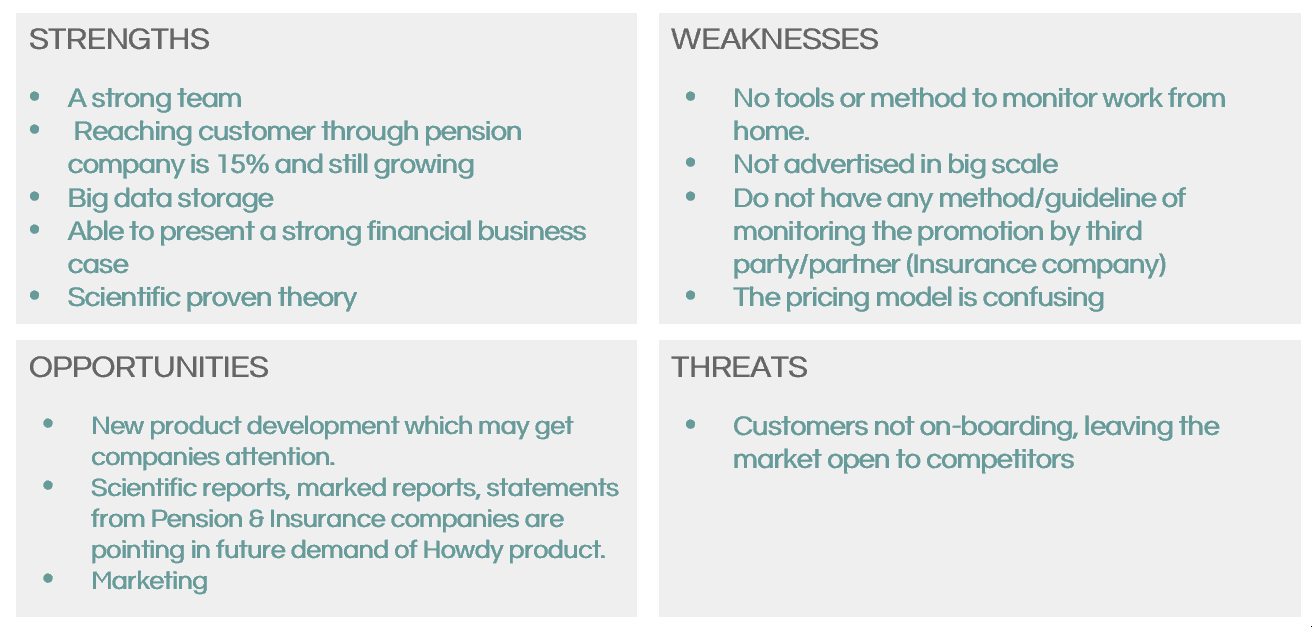
\includegraphics[width=0.95\textwidth]{figures/SWOT.png}
\caption{SWOT analysis describing the situation}
\end{figure}
To assess the position of Howdy we did a SWOT analysis to find out the company’s internal Strengths and Weaknesses as well as opportunities and threats from exterior forces with everything being based on the company presentation and other documents provided. The SWOT analysis helped us to find out what is working well, what is not, where Howdy should go, how they might get there and what might get in their way. This reduces the risk of failure, by understanding what Howdy is lacking, and eliminating hazards that might otherwise catch Howdy by surprise.

\noindent Howdy has a strong team of employees with a wide range of abilities. Their product is based on a scientifically proven theory to assess well-being. This theory is reviewed in more than 200 scientific studies since it was launched by Professor Per Bech, in 1998. Howdy has the capacity for big data and the system is scale-able as they use Microsoft Azure services. Howdy has a good relationship with their partners being the pension companies and healthcare providers.

\noindent Even though howdy has a strong team most of them are working from home and the management do not have any tools to monitor their performance. Furthermore, Howdy is not advertised on a big scale only through telemarketing, fairs and healthcare providers in exchange of an incentive which reduces the margin on Howdys product. They also do not have any control over how pension companies promoting as the pension companies are not allowed to.

\noindent Developing new products like for example Howdy Body can allow howdy to on-board customers in new segments like in this case where it is the blue collar industries where physical work is predominant. As statistics show that sick leaves are increasing in the workplace Howdys product should have increased demand in the future. Marketing on a big scale and directly to customers with an effective strategy should bring more business to howdy.

\noindent One of the threats that makes the company lose money is that customers are not on-boarding to a greater extend. This leaves the market open for competitors to acquire potential customers which will be a big problem as customers will be less likely to change to Howdy because of implementation costs.


\subsection{Porters generic strategies}
Porters generic strategies offers a way in which the managers can develop a business-level strategy that will facilitate a gain in competitive advantage\cite[p.190]{jones_george_2013}. Porter argues that choosing an appropriate strategy will help reduce and counter the threat of the five industry forces: rivalry among organizations, potential for entry, power of large suppliers and of large customers and the threat of substitute products\cite[p.189-190]{jones_george_2013}.\\
\noindent The information about their competitors offered by Howdy \cite{Extrainfo}, on top of what the previous model discussions revealed about the current strategy of the company, make it pretty clear that the company is going for a differentiation strategy. This type of strategy entails a way of distinguishing the products from those of the competition in one or more important dimensions\cite[p.191]{jones_george_2013}. According to the aforementioned information given by Howdy, they are differentiating by covering both healthy and sick employees and by being proactive, in contrast with the reactive strategy of their competitors. \\
\noindent In order to achieve a successful differentiation strategy according to Porter, the following things are needed: good Research \& Development team, the ability to deliver high-quality products and/or services and an effective sales and marketing team \cite{mind_tools_porter}. According to the results from the previously sections, it has been already identified that the companies current sales team is inefficient and from the company presentation\cite[s.11]{oneofthepresentations} it was revealed that daily tasks intervene with strategy meetings. The requirements for the differentiation strategy are thus not  fulfilled, which give insight into why the company has been loosing money for the past years. 

\subsection{Value proposition canvas}

The following model will provide Howdy with a tool to assess if the product is embracing the customer´s needs. In this particular case, the product is offering the companies, where white-collar employees are a resource, an instrument to defend them against factors that can cause sick leaves. Thus saving money for the company.

\noindent Howdy offers a \textit{service}, an IT platform, which helps companies to continuously monitor their employees´ health, through periodic questionnaires. The purpose of this aid is to assist companies in ‘\textit{customer job}: avoiding stress and burn-out of their staff. 
The problem emerges from the struggle, the \textit{pains}, to keep track of the psychological health, and furthermore, the lack of a \textit{"quick fix"} once the sickness has manifested. It is why Howdy offers solutions, \textit{pain relievers}, to the problem, by presenting periodic and generic questions about their status, and, when necessary, special support by qualified physiologists.    
By using this tool, companies don´t just improve their working environment, but they also achieve other \textit{gains}, like avoiding the cost of having a sick employee and ensuring better performance of the employees.


\subsection{Effectiveness/Efficiency}

As the 2019 situation is explored with the previously mentioned models, we can deduce that Howdy has a high effectiveness from the value proposition canvas, but is very inefficient. 

\begin{wrapfigure}{r}{0.3\textwidth}
\centering
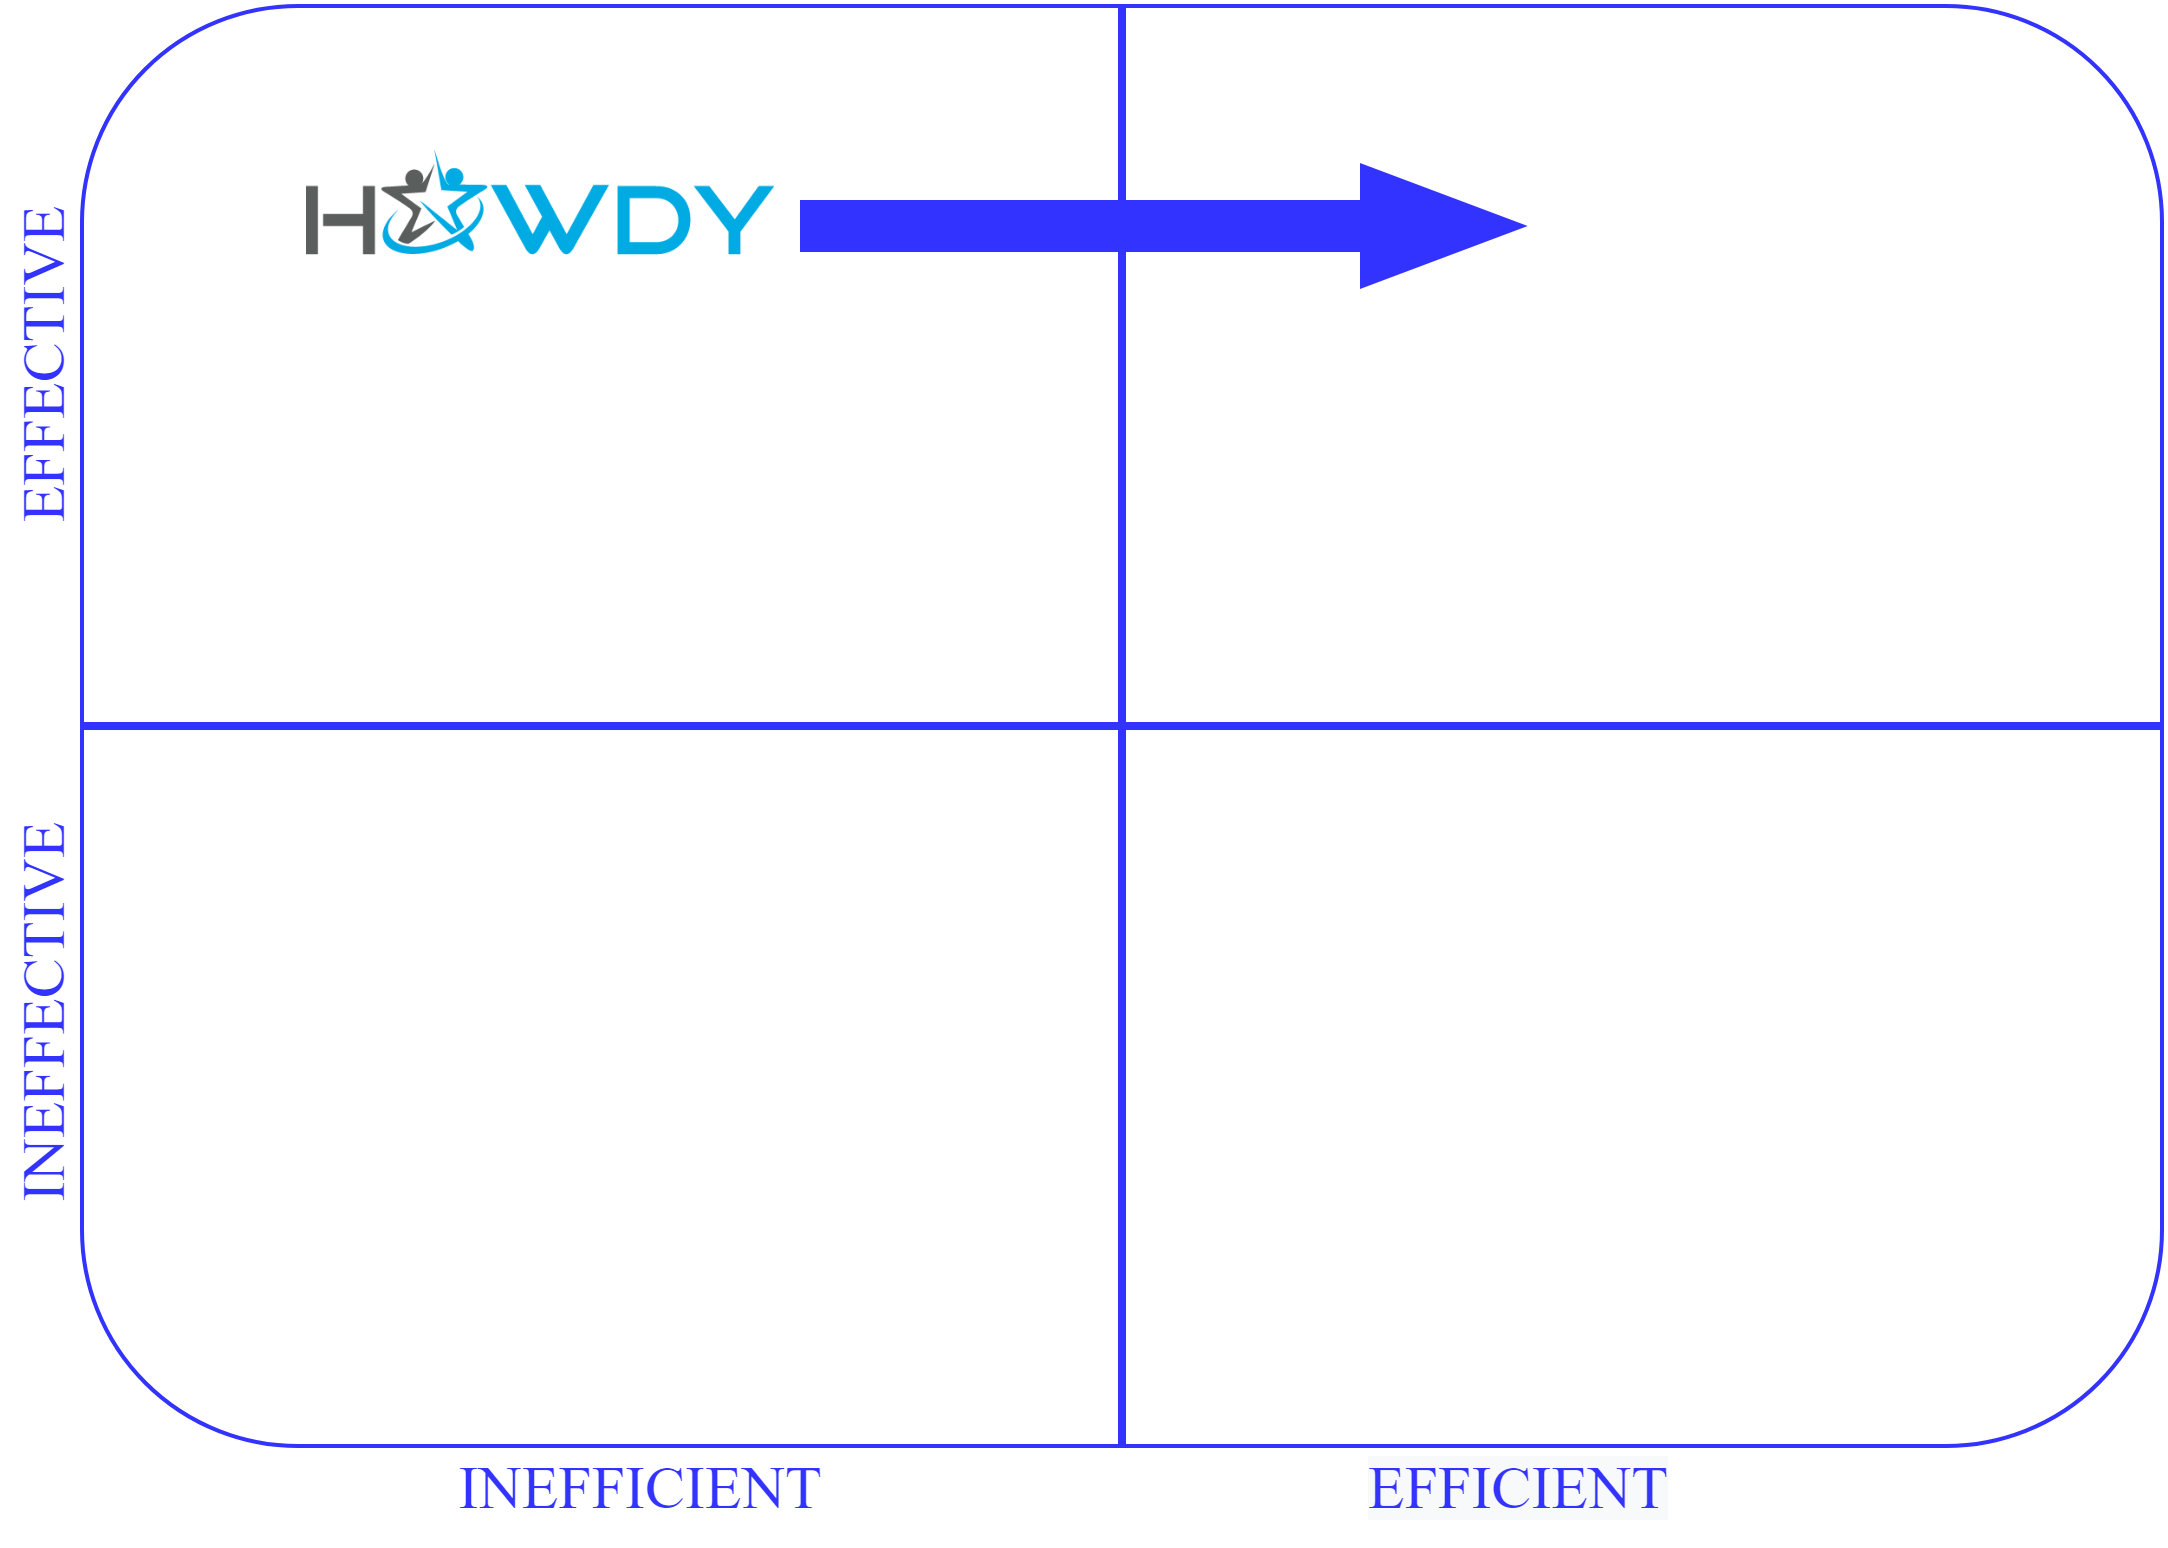
\includegraphics[width=0.3\textwidth]{figures/effiTEMO.png}
\caption{Effectiveness Efficiency, depicting the situation (2019) going towards the desired situation}
\label{fig:eff}
\end{wrapfigure}

\noindent In porters generic strategies, it was discussed how the daily tasks are interrupting strategy meetings, meaning that either the company is lacking resources or the managers are not distributing the resources in a productive way. Moreover, the company is using the health care providers as a way of advertisement by giving them a commission. This is proving to be inefficient since they are reducing their profit margins and they are not on-boarding enough customers, resulting in the company losing money.

\noindent The pension companies can also not legally advertise Howdy, they have it in their \textit{toolkit} and can be recommended to companies in that way, but it is not possible for Howdy to push their product, though that channel. This again tell us that the current marketing strategy is inefficient. 

\noindent From the analysis of the Effectiveness Efficiency model, it can be seen that Howdy pursues the right goal by developing an IT platform that make it easy to monitor the mental health of the employees and offering them help, but that the resources
are used poorly.This can be seen because Howdy is fulfilling their value proposition and they are adopting the right strategy of differentiation.

\noindent Our goal is to help the company move towards the far right corner of the model in figure \ref{fig:eff}, high efficiency/high effectiveness resulting in profits and a prosperous company. 


%%
%% Root cause analysis 
%%   -- jesper --
%%
\subsection{Root cause analysis}
Howdy is really focused on trying to prove their current product with a huge number of scientific papers and real-world performance statistics, but customers still do not buy their products. 

\noindent During our analysis we found multiple sub-problems and causes hereof; Howdy is not gaining enough customers through their partners due to relying on partners for marketing as seen in the BMC. Howdys´ partners are under strict regulations of what they can advertise to customers making it even harder for them to advertise Howdy. Furthermore Howdy is lacking resources in their sales department, making their current sales team very inefficient.

\noindent The SWOT analysis showed us that Howdy has scientific papers and research to back their statements along with powerful insurance partners. There’s plenty of opportunities for them to grow but yet fail to on-board more customers.

\noindent Using the SWOT analysis we found that Howdys' pricing model is confusing, intimidating and customers are unable to estimate the price of the product.

\noindent Our analysis enables us to define our key problem and problem owner. From the Value Proposition Canvas and Effectiveness/Efficiency model we can conclude that Howdy is effective  but very inefficient. Howdy tries to innovate and adapt to the market but they do not have a clear “focus” as explained in the porters generic strategy. Porters model furthermore tells us that Howdy tried to differentiate from the market, creating further distance to any external forces\cite[p.190]{jones_george_2013}.

\begin{wrapfigure}[3]{r}{2.5cm}
\centering

\includegraphics[scale=0.15]{figures/keyproblem.png}
\end{wrapfigure}
\paragraph{}

We conclude that the key problem is not successfully getting new clients and scaling the business, the symptoms of this is the company is losing money and struggle to profit.

\begin{wrapfigure}[8]{l}{5cm}
\centering
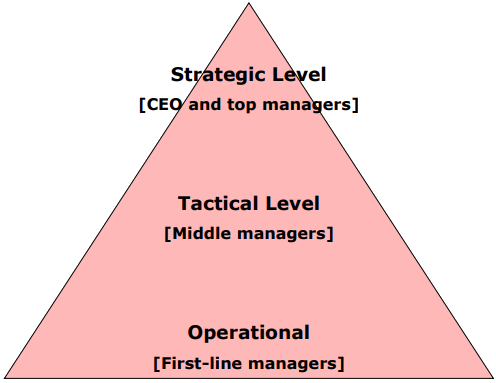
\includegraphics[scale=0.3]{figures/strategicallevel.png}
\caption{STO model}
\label{stomodel}
\end{wrapfigure}
\paragraph{}

We identified the key problem to be located at the strategical level as seen on [Figure \ref{stomodel}]. Making Rasmus Hartung (CEO) the key problem owner as he has the influence, money and trust from investors to implement the required proposed solutions due to the nature of the organization. That is not to say that he is alone, since he shares the blame with the following two employees: Gunnar Brabrand, the sales director, for not realizing the current marketing strategy is losing the company money and Mads Dørup (CTO) for failing to address the need for more maintenance personal at the tactical level.\newline


\noindent All our findings have been gathered in the Root cause tree [Figure \ref{rootcausetree}] to conclude the retrospective analysis. The Root Cause Tree starts with the key problem and breaks it down into sub-problems with causes. By doing this it becomes easier to get an overview of what needs to be solved for the given key problem to be eliminated. This means that, for Howdy, to get rid of their key problem, we have to solve all the causes. 

\begin{figure}[H]
\centering
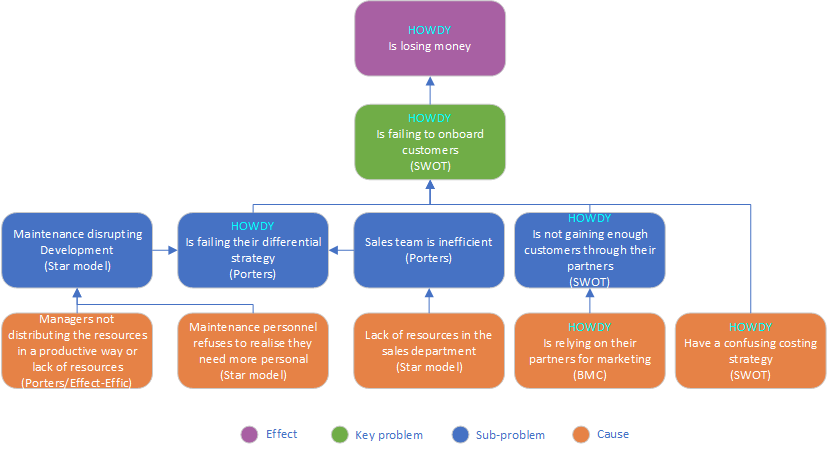
\includegraphics[scale=0.73]{figures/rootcause.png}
\caption{Root Cause Tree}
\label{rootcausetree}
\end{figure}


\newpage
\section{PART III : Prospective analysis}
% 6-8 pages !
% Propose and substantiate managerial, business and organisational solutions to the key problem(s):
% Proposals shall be prospective aiming at providing robust solutions to address the key problem(s).
% Remember to discuss the implementation aspect of your solution(s).
% There must be a coherence between the key problem(s), its causes and the proposed solutions.
% It is crucial to develop various alternative proposals for solutions. Select and motivate which proposals you think would best address the key problem.
% Use models and theories to support your proposals addressing organisational changes, changes of business model etc.

 \subsection{}
 
 
 % 

\newpage
\section{PART IV : Conclusions \& recommendations}
% 3-4 pages!
% • Present your recommendations based on your analysis
% • What would you recommend the company and the relevant actors to do?
% • How can your recommendations contribute to meet the challenge and give an edge to the competitive advantage of the company
% • Reflect on how your solution/recommendations can be implemented in the company
% • Describe how the key issues from your analysis and your recommendations are likely to affect the company from a strategic, tactical and operational level using your knowledge from the models and theories.
% • Identify and outline the possible extra information you need in order to implement your recommendations.


 \subsection{Modified Business canvas-Marco}


% BIBLIOGRAPHY
\newpage
\bibliographystyle{plain}
\bibliography{bibliography.bib}
%%%%%%%%%%%% Rapport %%%%%%%%%%%%%%%%%%%%%%%%%%


\end{document}

